\chapter{DESENVOLVIMENTO}\label{chap:desenvolvimento}



\section{Estudo do sensor, prototipagem, testes preliminares}

A revisão de literatura nos levou à escolha do modelo matemático mais simples que utiliza ângulos de Euler, embora possuindo diversas restrições no intervalo de validade, que também é o mais intuitivo~\cite{Stevens2016}. Para integração dos sinais na série temporal escolhemos o método trapezoidal pela relativa simplicidade de implementação.

Em relação ao equipamento, utilizamos, inicialmente, um sensor inercial modelo MPU-6050 (Figura~\ref{fig:mpu6050-sensor-top}) anexado a uma Raspberry Pi 3B (Figuras~\ref{fig:mpu6050-board-top}~e~\ref{fig:mpu6050-proto-top}):
\begin{figure}[H]
    \centering
    \caption{Sensor MPU-6050 encapsulado}\label{fig:mpu6050-sensor-top}
    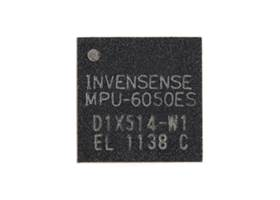
\includegraphics[width=0.5\textwidth]{figuras/mpu6050-sensor-top-straight.jpg}
    \fonte{o autor}
\end{figure}
A orientação dos sensores em relação ao encapsulamento obedece a regra da mão direita, conforme descrito na Figura~\ref{fig:mpu6050-diagram-axis}:
\begin{figure}[H]
    \centering
    \caption{Sensor MPU-6050 eixos em relação ao encapsulamento}\label{fig:mpu6050-diagram-axis}
    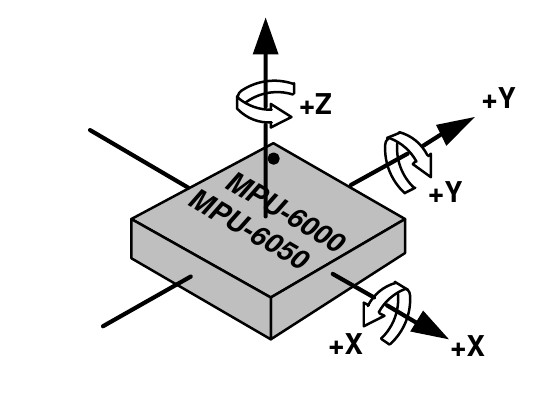
\includegraphics[width=0.5\textwidth]{figuras/mpu6050-diagram-axis.jpg}
    \fonte{\citeonline{mpu6050ps}}
\end{figure}
\begin{figure}[H]
    \centering
    \caption{Sensor MPU-6050 montado em placa módulo}\label{fig:mpu6050-board-top}
    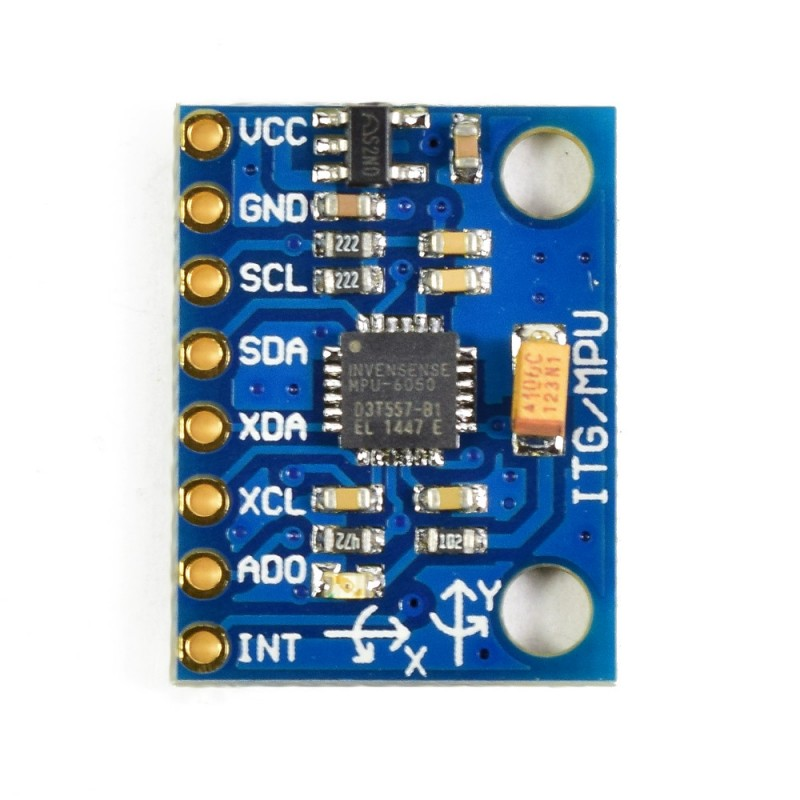
\includegraphics[width=0.5\textwidth]{figuras/mpu6050-board-top.jpg}
    \fonte{o autor}
\end{figure}
\begin{figure}[H]
    \centering
    \caption{Sensor MPU-6050 anexado à Raspberry Pi}\label{fig:mpu6050-proto-top}
    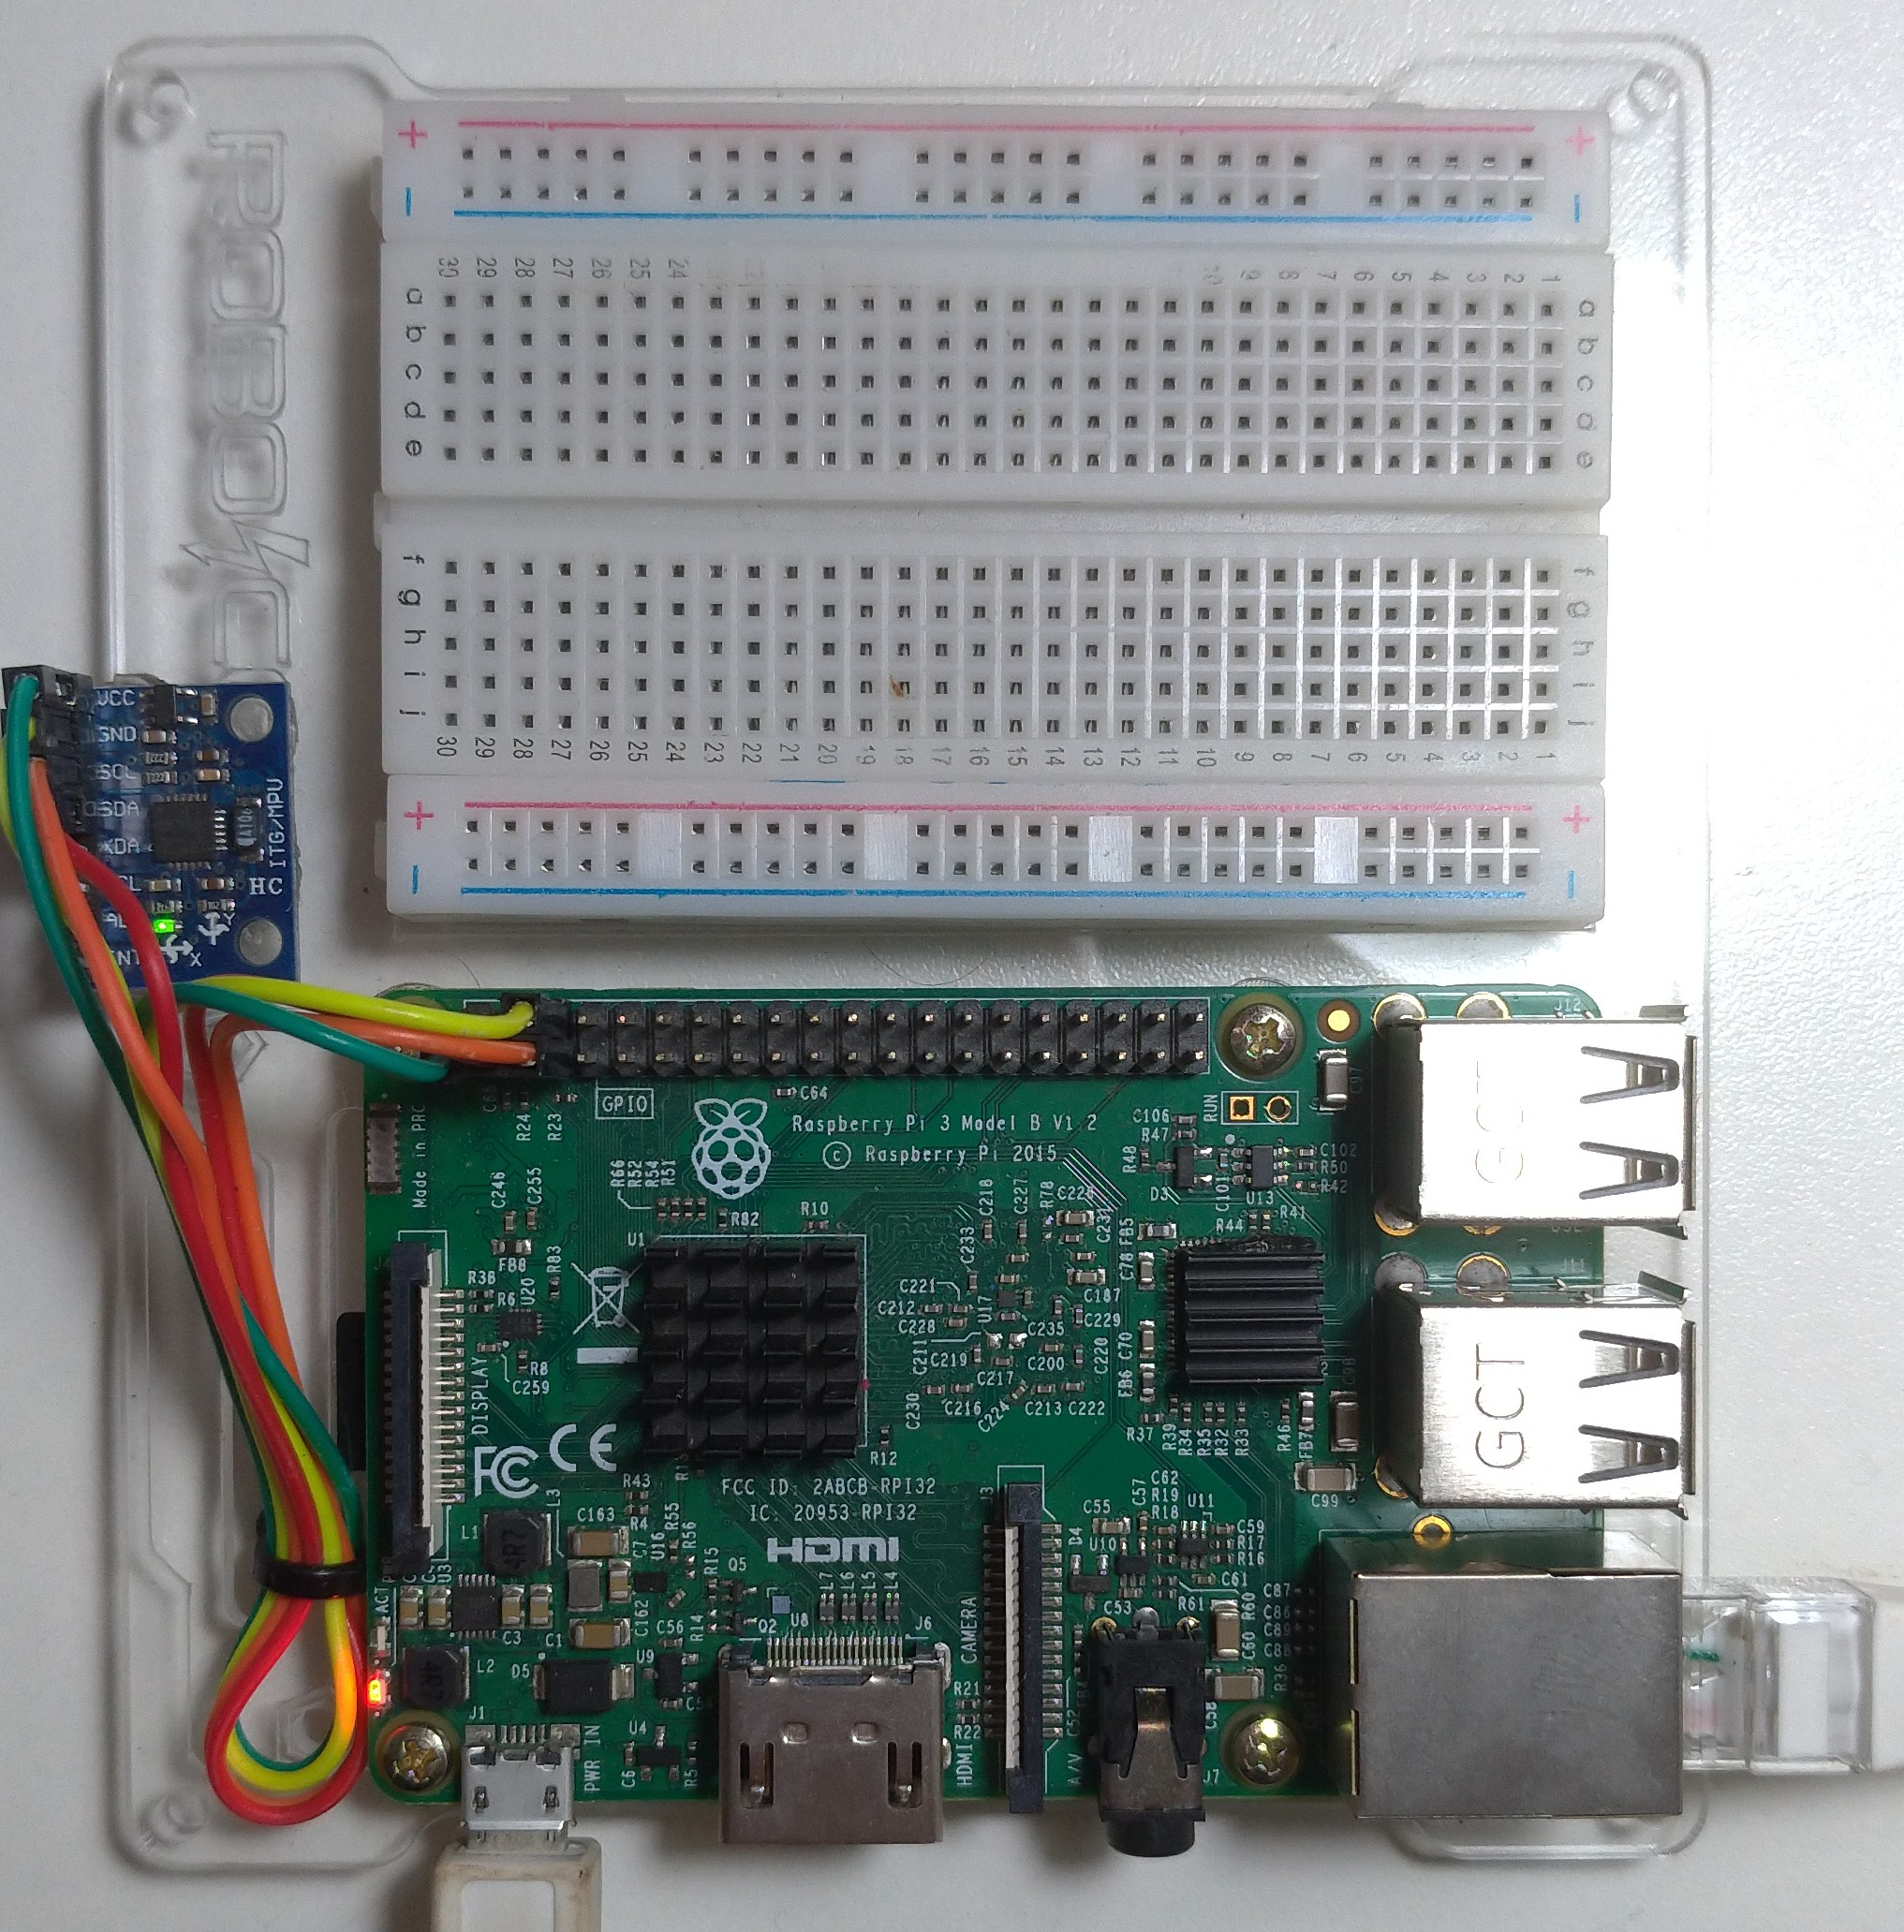
\includegraphics[width=0.5\textwidth]{figuras/mpu6050-proto-top.jpg}
    \fonte{o autor}
\end{figure}

Para a programação, utilizamos programação linguagem C para sistema Linux, com metologia ágil e desenvolvimento em código aberto. Nosso código consiste em duas peças distintas, um driver e uma aplicação de console para demonstração.

\section{Desenvolvimento de Software}

Para operar os sensores inerciais, consultamos extensamente a documentação do fabricante: Especificação do Produto~\cite{mpu6050ps} e Descrição e Mapa de Registradores~\cite{mpu6050rm}.

Destacamos que módulo MPU6050 possui três acelerômetros e três giroscópios, além de um sensor de temperatura, permite a coleta de dados de forma individual ou simultânea de todos os sensores, bem como oferece controle sobre a sensibilidade e o alcance das leituras dos acelerômetros e giroscópios, da taxa de amostragem, além de um filtro digital opcional.

A partir deles, estabelecemos como requisitos do sistema:
\begin{enumerate}
        \item obter dados simultâneos de todos os sensores em cada amostra,
        \item obter dados em intervalos regulares de tempo,
        \item obter dados em grandezas com significado físico,
        \item permitir o controle da sensibilidade dos sensores,
        \item permitir o controle da taxa de amostragem,
        \item permitir o controle das funções de filtro,
        \item seja utilizável com sistemas operacionais livres e amplamente disponíveis,
        \item possa ser instalado como um programa sem modificar o sistema operacional,
        \item possa ser livremente distribuído com licença de código aberto,
        \item possa ser operado pela linha de comando.
\end{enumerate}

Entretanto, não encontramos nenhuma solução pronta capaz de atender aos nossos requisitos. Nos restou, então, a partir dos manuais, desenvolver programas para controlar o sensor e obter os dados.

Os programas de nossa autoria foram escritos em linguagem C para sistemas Linux, rodam em uma \emph{Raspberry Pi 3B}, estão disponíveis\footnote{O driver em \href{https://www.github.com/ThalesBarretto/libmpu6050}{https://www.github.com/ThalesBarretto/libmpu6050}}\footnote{A aplicação em \href{https://www.github.com/ThalesBarretto/mpu6050}{https://www.github.com/ThalesBarretto/mpu6050}}sob licença permissiva de código aberto\footnote{Sob a ``MIT License'' disponível em \href{https://mit-license.org/}{https://mit-license.org/} e \href{https://opensource.org/licenses/MIT}{https://opensource.org/licenses/MIT}}, e acreditamos atender aos requisitos.

O driver em forma de biblioteca proporciona o controle das funções básicas dos sensores. Apenas as funções principais estão implementadas, como a coleta de dados simultânea em todos os eixos, o controle da taxa de amostragem, controle do filtro digital, inicialização, calibração e parada. O driver não inclui algumas funcionalidades específicas descritas pelo fabricante, como o controle de sensores secundários anexos, captura por disparo de interrupção, detecção de movimento e economia de energia. Entendemos que as funcionalidades ausentes não atendem diretamente aos propósitos do presente trabalho.

Por outro lado, o programa que demonstra a utilização das funções do driver e do controle dos sensores. A aplicação permite obter os dados na tela com escolha da taxa de amostragem e da sensibilidade dos sensores, bem como realizar calibração e inicialização, ou seja, as principais funções do nosso driver. A interface é do tipo linha de comando.

\section{Obtendo dados}

Na prática, os giroscópios  oferecem leituras de \(\mathbf{\omega}^{xyz}_{b/e}\), e os acelerômetros oferecem \(\mathbf{f}^{xyz}\), com eixos dos sensores, \(xyz\), alinhados aos sistemas \(frd\) e \(bf\), todos no quadro \(F^{b}\) do robô e situados no centro de massa. Fixamos um plano tangente à Terra no ponto \(Q\) de interesse, em que colocamos um sistema \(ned\) alinhado com o eixo ``abaixo'' alinhado ao vetor constante \(\mathbf{g}\), e um sistema \(tp\), e consideramos a Terra um referencial inercial (\(F^{i} \equiv F^{e}\equiv F^{tp}\)). Empregamos \(\mathbf{\Phi} \equiv \left[\phi \theta \psi \right]^T \) para descrever a atitude do corpo do robô utilizados ângulos de Euler na sequência anti-horária ``yaw'', ``pitch'', ``roll'' que levam do sistema \(ned\) ao sistema \(frd\).

A orientação do eixo dos sensores em relação ao corpo é fixa de tal modo que:

\begin{align*}
    {{C}_{frd/xyz}} &= {{C}_{xyz/frd}}  = \begin{bmatrix} 1 & 0 & 0 \\ 0 & -1 & 0 \\ 0 & 0 & -1 \end{bmatrix}
\end{align*}


Estabelecemos como condições iniciais, para o instante \(t_{0} = 0\):
\begin{align*}
    {\Phi} \left[0\right]
        &= \begin{bmatrix} 0 & 0 & 0 \end{bmatrix}^{T} \text{ (veículo nivelado)} \\
    {^{e}{\mathbf{p}^{tp}_{cm/Q}}\left[0\right]}
    &= \begin{bmatrix} 0 & 0 & 0 \end{bmatrix}^{T} \text{ (situado na origem do plano tangente)} \\
    {^{e}{\dot{\mathbf{p}}^{tp}_{cm/Q}}\left[0\right]}
    &= \begin{bmatrix} 0 & 0 & 0 \end{bmatrix}^{T} \text{ (em repouso)} \\
\end{align*}

Utilizamos os giroscópios para obter:
\begin{align*}
     &\mathbf{\omega}^{frd}_{b/e}{\left[k\right]}
     = C_{frd/xyz} \mathbf{\omega}^{xyz}_{b/e}{\left[k\right]}
        \equiv \begin{bmatrix} P{\left[k\right]} & Q{\left[k\right]} & R{\left[k\right]} \end{bmatrix}^{T}
        \text{} \\
\end{align*}

Podemos obter a atitude integrando numericamente:
\begin{align*}
{\Phi}{\left[ k \right]}
    &\approx {\Phi} {\left[ k-1 \right]} + T {\dot{\Phi}{\left[ k -1 \right]}} \\
    &\approx {\Phi} {\left[ k-1 \right]} + T {\left( H {\left( \Phi{\left[ k-1 \right]} \right)}{\mathbf{\omega}^{frd}_{b/e}}{\left[ k-1 \right]}\right)} \\
\end{align*}

Quando \((\mathbf{a} \approx 0)\), \((\lvert\mathbf{f}\lvert \approx \lvert\mathbf{g}\lvert)\), podemos obter \(\theta\) e \(\phi\) dos acelerômetros:
\begin{align*}
    {\phi}\left[k\right] &=  \textrm{atan2}\left(\frac{\mathbf{-f}_{y}}{\mathbf{-f}_{z}}\right),\quad
    -\pi  < \phi \leq \pi \\
    {{\theta}{\left[k\right]}} &= \textrm{atan2} \left( {\frac{-\mathbf{f}_{x}\left[k\right] }{ \sqrt{ {\left({{-\mathbf{f}_{y}^{2}}\left[k\right]}\right)} + {\left({{-\mathbf{f}}_{z}^{2}}{\left[k\right]}\right)}}}} \right), \quad -\frac{\pi}{2} \leq \theta \leq \frac{\pi}{2} \\
\end{align*}

Os acelerômetros fornecem diretamente \(\mathbf{f}^{bf}\), e, indiretamente, \(\mathbf{a}\):
\begin{align*}
    \mathbf{a} &= \dfrac{\mathbf{F}}{m} + \mathbf{G} \equiv \mathbf{f} - \mathbf{g} \\
{^{i}\mathbf{a}^{tp}_{cm/Q}\left[k\right]} &= C_{tp/frd}\left[k\right]{^{i}\mathbf{f}^{frd}_{cm/Q}\left[k\right]} - \mathbf{g}^{tp} \\
\end{align*}

Empregando as transformações de coordenadas, chegamos em:
\begin{align*}
    \mathbf{a} &=
    \begin{bmatrix}
        {{\mathbf{f}_{x}} {c\psi} {c\theta}}
        + {{\mathbf{f}_{y}} {\left( -{s\phi} {s\theta} {c\psi} + {s\psi} {c\phi} \right)}}
        + {{\mathbf{f}_{z}} {\left( -{s\phi} {s\psi} - {s\theta} {c\phi} {c\psi} \right)}} \\
        {{\mathbf{f}_{x}} {s\psi} {c\theta}}
        + {{\mathbf{f}_{y}} {\left(-{s\phi} {s\psi} {s\theta} - {c\phi} {c\psi} \right)}}
        + {{\mathbf{f}_{z}} {\left( {s\phi} {c\psi} - {s\psi} {s\theta} {c\phi} \right)}} \\
        - {{\mathbf{f}_{x}} {s\theta}}
        - {{\mathbf{f}_{y}} {s\phi} {c\theta}}
        - {{\mathbf{f}_{z}} {c\phi} {c\theta}}
        - {\mathbf{g}_{d}} 
    \end{bmatrix}  \\
\end{align*}
\begin{equation*}
    \mathbf{f}^{frd} =
    \begin{bmatrix}
    {\mathbf{f}_{x}} \\
    -{\mathbf{f}_{y}} \\
    -{\mathbf{f}_{z}}
    \end{bmatrix}
    \text{,}\quad
    \mathbf{g}^{frd} =
    \begin{bmatrix}
    -{{\mathbf{g}_{d}} {s\theta}} \\
    {{\mathbf{g}_{d}} {s\phi} {c\theta}} \\
    {{\mathbf{g}_{d}} {c\phi} {c\theta}}
    \end{bmatrix}
    \text{,}\quad
    \mathbf{a}^{frd} =
    \begin{bmatrix}
      {\mathbf{f}_{x}} + {{\mathbf{g}_{d}} {s\theta}} \\
    - {\mathbf{f}_{y}} - {{\mathbf{g}_{d}} {s\phi} {c\theta}} \\
    - {\mathbf{f}_{z}} - {{\mathbf{g}_{d}} {c\phi} {c\theta} }
    \end{bmatrix}
\end{equation*}


Por último, utilizamos os resultados para integrar a posição:
\begin{align*}
    {^{e}{\dot{\mathbf{v}}}^{tp}_{cm/e}{\left[k\right]}}
        &\approx {^{a}{\dot{\mathbf{v}}}^{tp}_{cm/e}}{\left[ k-1 \right]}
        + T \Big( {C_{tp/frd}\left({\Phi}{\left[ k-1 \right]} \right)} {{\mathbf{f}}^{frd}\left[k-1\right]} {-{\mathbf{g}}^{tp}} \Big) \\
    {^{e}{\mathbf{p}^{tp}_{cm/Q}}\left[k\right]}
    &\approx     {^{e}{\mathbf{p}^{tp}_{cm/Q}}\left[k-1\right]}
    + T \Big( {^{e}\mathbf{v}^{tp}_{cm/Q}{\left[ k-1 \right]}} \Big) \\
\end{align*}


\section{Fusão de sensores}

No nosso caso, podemos utilizar um filtro complementar, bastante simples, para calcular a atitude. O filtro consiste em utilizar simultaneamente dois métodos para obter a estimativa de atitude: a integração das taxas angulares e o cálculo da atitude a partir dos acelerômetros. Ao resultado de cada método é atribuído um peso que representa sua confiabilidade naquele instante, ambos são somados e o resultado final é normalizado. Em sendo detectado um movimento de aceleração, utilizamos apenas os giroscópios para determinar a atitude.

Desse modo podemos evitar os resultados divergentes da simples integração de giroscópios e ao mesmo tempo reduzir as oscilações da estimativa pelo ruído dos acelerômetros, o que acaba funcionando como um mecanismo de estabilização das estimativas de atitude.

\section{Testes de bancada para coleta de dados}

Para analisar a viabilidade e a resposta do sistemas e métodos, propomos a realização de testes de bancada em condições controladas para comparar os resultados obtidos com resultados esperados. Pretendemos realizar teste estáticos e testes cinemáticos, com os sensores em posição estacionária ou em movimento, respectivamente.
